\iffalse
\documentclass[]{article}
\usepackage{amsfonts, amssymb, amsmath}
\usepackage{float}
\usepackage{graphicx}

\title{Question 9.3.7}
\author{Anupama Kulshreshtha \\ EE22BTECH11009}
\date{}
\begin{document}
\maketitle
\providecommand{\pr}[1]{\ensuremath{\Pr\left(#1\right)}}
\providecommand{\prt}[2]{\ensuremath{p_{#1}^{\left(#2\right)} }}        % own macro for this question
\providecommand{\qfunc}[1]{\ensuremath{Q\left(#1\right)}}
\providecommand{\sbrak}[1]{\ensuremath{{}\left[#1\right]}}
\providecommand{\lsbrak}[1]{\ensuremath{{}\left[#1\right.}}
\providecommand{\rsbrak}[1]{\ensuremath{{}\left.#1\right]}}
\providecommand{\brak}[1]{\ensuremath{\left(#1\right)}}
\providecommand{\lbrak}[1]{\ensuremath{\left(#1\right.}}
\providecommand{\rbrak}[1]{\ensuremath{\left.#1\right)}}
\providecommand{\cbrak}[1]{\ensuremath{\left\{#1\right\}}}
\providecommand{\lcbrak}[1]{\ensuremath{\left\{#1\right.}}
\providecommand{\rcbrak}[1]{\ensuremath{\left.#1\right\}}}
\newcommand{\sgn}{\mathop{\mathrm{sgn}}}
\providecommand{\abs}[1]{\left\vert#1\right\vert}
\providecommand{\res}[1]{\Res\displaylimits_{#1}} 
\providecommand{\norm}[1]{\left\lVert#1\right\rVert}
%\providecommand{\norm}[1]{\lVert#1\rVert}
\providecommand{\mtx}[1]{\mathbf{#1}}
\providecommand{\mean}[1]{E\left[ #1 \right]}
\providecommand{\cond}[2]{#1\middle|#2}
\providecommand{\fourier}{\overset{\mathcal{F}}{ \rightleftharpoons}}
\newenvironment{amatrix}[1]{%
  \left(\begin{array}{@{}*{#1}{c}|c@{}}
}{%
  \end{array}\right)
}
%\providecommand{\hilbert}{\overset{\mathcal{H}}{ \rightleftharpoons}}
%\providecommand{\system}{\overset{\mathcal{H}}{ \longleftrightarrow}}
	%\newcommand{\solution}[2]{\textbf{Solution:}{#1}}
\newcommand{\solution}{\noindent \textbf{Solution: }}
\newcommand{\cosec}{\,\text{cosec}\,}
\providecommand{\dec}[2]{\ensuremath{\overset{#1}{\underset{#2}{\gtrless}}}}
\newcommand{\myvec}[1]{\ensuremath{\begin{pmatrix}#1\end{pmatrix}}}
\newcommand{\mydet}[1]{\ensuremath{\begin{vmatrix}#1\end{vmatrix}}}
\newcommand{\myaugvec}[2]{\ensuremath{\begin{amatrix}{#1}#2\end{amatrix}}}
\providecommand{\rank}{\text{rank}}
\providecommand{\pr}[1]{\ensuremath{\Pr\left(#1\right)}}
\providecommand{\qfunc}[1]{\ensuremath{Q\left(#1\right)}}
	\newcommand*{\permcomb}[4][0mu]{{{}^{#3}\mkern#1#2_{#4}}}
\newcommand*{\perm}[1][-3mu]{\permcomb[#1]{P}}
\newcommand*{\comb}[1][-1mu]{\permcomb[#1]{C}}
\providecommand{\qfunc}[1]{\ensuremath{Q\left(#1\right)}}
\providecommand{\gauss}[2]{\mathcal{N}\ensuremath{\left(#1,#2\right)}}
\providecommand{\diff}[2]{\ensuremath{\frac{d{#1}}{d{#2}}}}
\providecommand{\myceil}[1]{\left \lceil #1 \right \rceil }
\newcommand\figref{Fig.~\ref}
\newcommand\tabref{Table~\ref}
\newcommand{\sinc}{\,\text{sinc}\,}
\newcommand{\rect}{\,\text{rect}\,}
%%
%	%\newcommand{\solution}[2]{\textbf{Solution:}{#1}}
%\newcommand{\solution}{\noindent \textbf{Solution: }}
%\newcommand{\cosec}{\,\text{cosec}\,}
%\numberwithin{equation}{section}
%\numberwithin{equation}{subsection}
%\numberwithin{problem}{section}
%\numberwithin{definition}{section}
%\makeatletter
%\@addtoreset{figure}{problem}
%\makeatother

%\let\StandardTheFigure\thefigure
\let\vec\mathbf

There are 5\% defective items in a large bulk of items. What is the probability 
that a sample of 10 items will include not more than one defective item?
\solution
\fi
\begin{table}[!ht]
\centering
\begin{tabular}{|l|c|r|}
    \hline
    Parameter & Values & Description\\
    \hline
    $n$ & 10 & Number of items\\
    \hline
    $p$ & 0.05 & Probability of being defective\\
    \hline
    $q$ & 0.95 & Probability of not being defective\\
    \hline
    $\mu = np$ & 0.5 & Mean\\
    \hline
    ${\sigma}^2 = npq$ & 0.475 & Variance\\
    \hline
\end{tabular}
\caption{Definition of parameters and their values}
\label{tab:gaussian/9/3/7}
\end{table}
\begin{enumerate}
\item Binomial:
The cdf using binomial is given by  
\begin{align}
	F_Y\brak{n} &= \Pr(Y \leq n) \\
        &= \sum_{k=0}^n\comb{10}{k}p^k\brak{1-p}^{10-k}
\end{align}
We require $\Pr(Y \leq 1)$. Since $n = 1$,
\begin{align}
	F_Y\brak{1} &= \Pr(Y \leq 1) \\
        &=  \sum_{k=0}^1\comb{10}{k}(0.05)^k\brak{0.95}^{10-k} \\
	&= 0.9138 
	\label{eq:9371}
\end{align}
\item Gaussian:
$Y \sim \mathcal{N}\brak{\mu, \sigma^2}$\\
To obtain cdf,
\begin{align}
\Pr(Y \leq 1) &= F_Y\brak{1}\\
F_Y\brak{x} &= \Pr(Y \leq x)\\
&= \Pr(Y - \mu \leq x - \mu)\\
&= \Pr(\frac{Y - \mu}{\sigma} \leq \frac{x - \mu}{\sigma})\\
&= 1 - \Pr(\frac{Y - \mu}{\sigma} > \frac{x - \mu}{\sigma})
\end{align}
We know that,
\begin{align}
\frac{Y - \mu}{\sigma} \sim \mathcal{N}\brak{0, 1}\\
\Pr(X > x) &= \qfunc{x}
\end{align}
Hence,
\begin{align}
F_Y\brak{x} &= 1 - \qfunc{\frac{x - \mu}{\sigma}}, \text{if $x > \mu$}\\
&= \qfunc{\frac{\mu - x}{\sigma}}, \text{if $x < \mu$}\\
\implies F_Y\brak{1} &= 1 - \qfunc{\frac{0.5}{\sqrt{0.475}}}\\
&= 0.766
\end{align}
With correction of 0.5,
\begin{align}
\Pr(Y \leq 1.5) &= F_Y\brak{1.5}\\
F_Y\brak{1.5} &= 1 - \qfunc{\frac{1}{\sqrt{0.475}}}\\
&= 0.927
\label{eq:9372}
\end{align}
From \eqref{eq:9371} and \eqref{eq:9372}
\begin{align}
\Pr(Y \leq 1) \approx F_Y\brak{1.5}
\end{align}
\begin{table}[!ht]
\centering
\begin{tabular}{|l|c|r|}
    \hline
    Binomial & Gaussian (without correction) & Gaussian (with correction)\\
    \hline
    0.9138 & 0.766 & 0.927\\
    \hline
\end{tabular}
\caption{Probability obtained using different methods}
\label{tab:gaussian/9/3/7/1}
\end{table}
\begin{figure}[!ht]
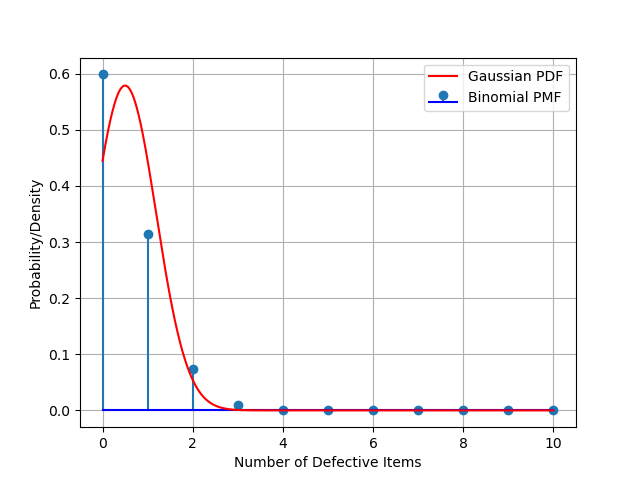
\includegraphics[width=\columnwidth]{./figs/fig.png}
\caption{Binomial pmf vs Gaussian pdf}
\label{fig:gaussian/9/3/7/2}
\end{figure}
\end{enumerate}
